\documentclass[12pt,a4paper]{article}
\usepackage{geometry}
\usepackage[utf8]{inputenc}
\usepackage{graphicx}
\usepackage{float}
\usepackage[most]{tcolorbox}
\usepackage[spanish,es-noshorthands]{babel}
\usepackage{titlesec}
\usepackage{hyperref}
\titleformat*{\section}{\large\bfseries}

\title{Sistemas Operativos \\\ Gestión de la Memoria}
\author{Acosta Quintana Lautaro Alejo}
\geometry {
    left=1.59 cm,
    right=1.58 cm,
    tmargin=1.9 cm,
    bottom=2.534 cm
}
\begin{document}
\maketitle
\tableofcontents
\break

El sistema operativo es el encargado de la tarea de subdivisión y a esta tarea se le denomina \textbf{gestión de la memoria} .
\section{Requisitos de la Gestión de la Memoria}
La gestión de la memoria debe satisfacer los siguientes requisitos:
\begin{itemize}
    \item Reubicación.
    \item Protección.
    \item Compartición.
    \item Organización Lógica.
    \item Organización Física.
\end{itemize}
\subsection{Reubicación}
Es necesario poder intercambiar procesos en la memoria principal para maximizar la utilización del procesador y si una vez que el programa se ha llevado al disco, solo pudiera ser colocado otra vez en la misma región donde estaba, esto sería contraproducente. Por lo que es necesario poder \textbf{reubicarlo} en un área de memoria diferente (esto posible gracias al intercambio o \textit{swap}).\\\\ 
\begin{figure}[H]
    \centering
    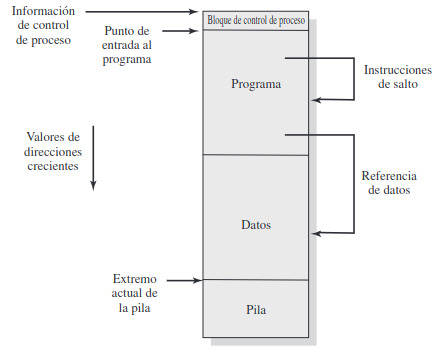
\includegraphics[width=10cm]{proceso1.jpeg}\par
    \caption{Requisitos de direccionamiento para un proceso}
\end{figure}
El sistema operativo necesita conocer la ubicación de la información de control del proceso y de la pila de ejecución, así como el punto de entrada que utiliza el proceso para iniciar la ejecución (Estas direcciones son fáciles de conseguir, ya que es el sistema operativo el encargado de traer el proceso a la memoria principal). Sin embargo, el hardware del procesador y el software del sistema operativo tendrán que ser capaces de traducir las referencias de memoria encontradas en el código del programa en direcciones de memoria físicas, que reflejen la ubicación actual del programa en la memoria principal.
\subsection{Protección}
Los programas de otros procesos no deben ser capaces de referenciar sin permiso posiciones de memoria de un proceso, tanto en modo lectura como escritura. Todas las referencias de memoria generadas por un proceso deben comprobarse en tiempo de ejecución para poder asegurar que se refieren solo al espacio de memoria asignado a dicho proceso. El procesador debe ser capaz de abortar tales instrucciones en el punto de ejecución.\\\\
Los requisitos de protección de memoria deben ser satisfechos por el procesador en lugar del sistema operativo, ya que el sistema operativo no podría anticiparse a todas las referencias que el programa hará e incluso, si fuera posible, sería muy costoso el cálculo para comprobarlos.

\begin{tcolorbox}[colback=cyan!10, colframe=blue!70, title=Nota]
    Solo es posible evaluar la permisibilidad de una referencia (acceso a datos o salto) en tiempo de ejecución de la instrucción que realiza dicha referencia.
\end{tcolorbox}
\subsection{Compartición}
Cualquier mecanismo de protección debe permitir a varios procesos acceder a la misma porción de memoria principal. El sistema de gestión de memoria debe permitir el acceso controlado a áreas de memoria compartidas sin comprometer la protección esencial.
\subsection{Organización Lógica}
La memoria principal de un computador se organiza como un espacio de almacenamiento lineal o unidimensional, compuesto por una secuencia de bytes o palabras. A nivel físico, la memoria secundaria está organizada de forma similar. En cambio, la mayoría de los programas se organizan en módulos (que pueden ser modificables o no).\\\\ 
Si el sistema operativo y el hardware del computador pueden tratar de forma efectiva los programas de usuarios y los datos en la forma de módulos, se logran las siguientes ventajas:
\begin{enumerate}
    \item Los módulos se pueden escribir y compilar independientemente, con todas las referencias de un módulo desde otro, resueltas por el sistema en tiempo de ejecución.
    \item Con una sobrecarga adicional, se puede proporcionar grados de protección a los módulos (solo lectura, solo ejecución).
    \item Es posible introducir mecanismos por los cuales los módulos se pueden compartir entre los procesos. La ventaja de esto es que corresponde con la forma en la que el usuario ve el problema, por lo que es más fácil para el especificar la compartición deseada.
\end{enumerate}
\begin{tcolorbox}[colback=cyan!10, colframe=blue!70, title=Nota]
    La herramienta más adecuada para estos requisitos es la \textbf{segmentación} .
\end{tcolorbox}

\subsection{Organización Física}
La organización del flujo de información entre la memoria principal y secundaria supone una de las preocupaciones principales del sistema. La responsabilidad para este flujo podría asignarse a cada programar, pero no es deseable o incluso practicable por dos motivos:
\begin{enumerate}
    \item La memoria principal disponible para un programa podría ser insuficiente. En este caso tendría que usarse \textbf{\textit{overlaying}} (\textbf{superposición}) en la cual los programas y sus datos se organizan de manera que pueda asignarse la misma región de memoria a varios módulos, con un programa principal responsables de intercambiar los módulos entre disco y memoria. La programación con \textit{overlay} malgasta tiempo del programador.
     \item En un entorno multiprogramado, el programador no conoce en tiempo de codificación cuánto espacio estará disponible o dónde se localizará dicho espacio.
\end{enumerate}
La tarea de mover la información entre los dos niveles de memoria debería ser una responsabilidad del sistema.

\section{Particionamiento de la Memoria}
La operación principal de la gestión de la memoria es traer los procesos a la memoria principal para que el procesador los pueda ejecutar. Una de estas técnicas es el particionamiento.
\subsection{Particionamiento Fijo}
El esquema más simple para gestionar la memoria disponible es repartir en regiones con límites fijos.
\subsubsection{Tamaños de partición}
\begin{figure}[H]
    \centering
    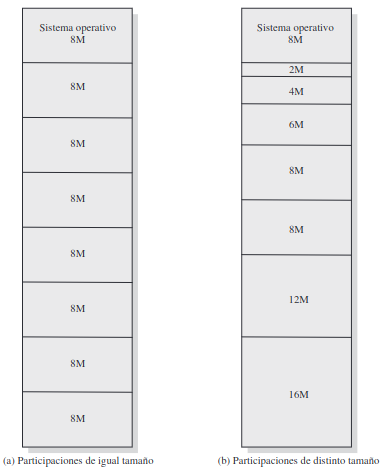
\includegraphics[width=10cm]{particionfija.png}\par
    \caption{Ejemplo de particionamiento fijo en una memoria de 64 MB}
\end{figure}
Existen dos alternativas para el particionamiento fijo. Una consiste en hacer uso de particiones del mismo tamaño; en este caso cualquier proceso con tamaño menor o igual puede cargarse en la partición disponible. Si todas las particiones están llenas y no hay ningún proceso en estado Listo o Ejecutando, el sistema puede mandar a \textit{swap} un proceso de cualquier partición y cargar otro. Existen dos dificultades con esta estrategia:
\begin{itemize}
    \item Un programa puede ser demasiado grande para entrar en una partición. En este caso el programador debe diseñar el programa con uso de \textit{overlays}. Cuando se necesita un módulo que no está presente, el programa de usuario debe cargar dicho módulo en la partición del programa superponiéndolo (\textit{overlaying}) a cualquier programa o dato que haya allí.
    \item La utilización de la memoria principal es extremadamente ineficiente. Este fenómeno, en el cual hay espacio interno malgastado debido al hecho de que el bloque de datos cargado es menor que la partición, se conoce como \textbf{fragmentación interna} .
\end{itemize}
Ambos problemas se pueden mejorar pero no resolver, utilizando particiones de tamaño diferente.
\subsubsection{Algoritmo de ubicación}
\begin{figure}[H]
    \centering
    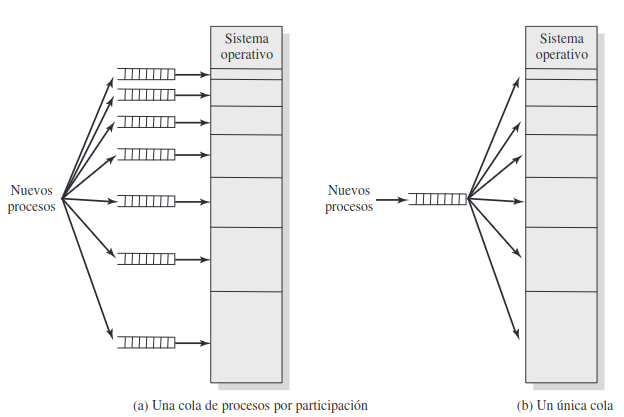
\includegraphics[width=12cm]{particionfija2.png}\par
    \caption{Asignación de memoria para particionamiento fijo.}
\end{figure}
Con particiones del mismo tamaño, la ubicación de los procesos en memoria es trivial.\\\\ 
Con particiones de diferentes tamaños, hay dos formas de asignar los procesos a las particiones. \\ 
\begin{itemize}
    \item Asignar cada proceso a la partición más pequeña dentro de la que cabe. En este caso se utiliza una cola de planificación para cada partición, que mantenga procesos en disco destinados a dicha partición. La ventaja de esta técnica es que se minimiza la \textbf{fragmentación interna}, aunque no es óptima para un sistema complejo. Se asume que se conoce el tamaño máximo de memoria que un proceso requerirá, en caso contrario, la única alternativa es un esquema de \textit{overlays} o usar memoria virtual. Es la técnica más sencilla.
    \item Emplear una única cola para todos los procesos. En el momento de cargar un proceso en la memoria principal, se selecciona la partición más pequeña disponible capaz de albergar a dicho proceso.
\end{itemize}
Si todas las particiones están ocupadas, se debe llevar a cabo una decisión para enviar a \textit{swap} algún proceso.
\begin{tcolorbox}[colback=cyan!10, colframe=blue!70, title=Nota]
    Tiene preferencia a la hora de ser expulsado a disco el proceso que ocupe la partición más pequeña que pueda albergar al proceso entrante.
\end{tcolorbox}
\subsection{Particionamiento Dinámico}
Con particionamiento dinámico, las particiones son de longitud y número variable. Cuando se lleva un proceso a la memoria principal, se le asigna exactamente tanta memoria como requiera.
\begin{figure}[H]
    \centering
    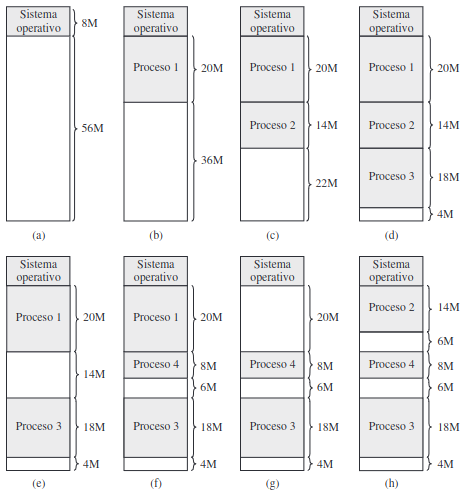
\includegraphics[width=12cm]{particiondinamica.png}\par
    \caption{El efecto del particionamiento dinámico.}
\end{figure}
Como se observa en la Figura 4., el método comienza correctamente, pero lleva a una situación en la cual existen muchos huecos pequeños en la memoria. A medida que pasa el tiempo, la memoria se fragmenta cada vez más y la utilización decrementa. Este fenómeno se conoce como \textbf{fragmentación externa}, indicando que la memoria que es externa a todas las particiones se fragmenta de forma incremental.\\\\ 
Una técnica para eliminar la fragmentación externa es la \textbf{compactación}: de vez en cuando, el sistema operativo desplaza los procesos en memoria, de forma que se encuentren contiguos y de este modo toda la memoria libre se encontrará unida en un bloque. La desventaja de la compactación es que se trata de un procedimiento que consume tiempo y recursos del procesador.
\begin{tcolorbox}[colback=cyan!10, colframe=blue!70, title=Nota]
    La compactación requiere la capacidad de \textbf{reubicación dinámica} (mover un programa desde una región a otra en la memoria principal sin invalidar las referencias de memoria de cada programa).
\end{tcolorbox}
\subsubsection{Algoritmo de ubicación}
Tres algoritmos de colocación que pueden considerarse son \textit{best-fit}, \textit{first-fit}, \textit{next-fit} y \textit{worst-fit}; todos limitas a elegir entre los bloques libres de la memoria principal que son iguales o más grandes que el proceso que va a llevar a la memoria. 
\begin{itemize}
    \item \textbf{Best-fit} elige el bloque más cercano en tamaño a la petición.
    \item \textbf{First-fit} comienza a analizar la memoria desde el principio y escoge el primer bloque disponible que sea suficientemente grande.
    \item \textbf{Next-fit} comienza a analizar la memoria desde la última colocación y elige el siguinete bloque disponible que sea suficientemente grande.
    \item \textbf{Worst-fit} elige el mayor bloque de memoria libre para un proceso.
\end{itemize}
\begin{tcolorbox}[colback=cyan!10, colframe=blue!70, title=Nota]
    Cuál técnica es mejor depende de la secuencia exacta de intercambio y tamaño de los procesos. Algunos comentarios son:
    \begin{itemize}
        \item First-fit es el más sencillo y normalmente es el mejor y más rápido.
        \item Next-fit tiende a producir resultados ligeramente peores que First-fit.
        \item Next-fit lleva más frecuentemente a una asignación de un bloque libre al final de la memoria el cual normalmente es el bloque más grande de memoria libre, lo que lleva a que se divida en pequeños fragmentos y requiera más frecuentemente la compactación.
        \item First-fit puede dejar el final del espacio de almacenamiento con pequeñas particiones libres que necesitan buscarse en cada paso del primer ajuste siguiente.
        \item Best-fit tiene normalmente el peor comportamiento, debido a que busca el bloque más pequeño que satisfaga la petición garantiza que el fragmento que quede sea lo más pequeño posible. Por esto la compactación debe realizarse con mayor frecuencia que en el resto de algoritmos.
    \end{itemize}
\end{tcolorbox}
\subsubsection{Algoritmo de reemplazamiento}
En un sistema multiprogramado, puede ocurrir que todos los procesos de la memoria principal estén en estado bloqueado y no haya suficiente memoria para un proceso adicional, incluso después de una compactación. Para evitar malgastar tiempo del procesador, el sistema operativo intercambiará alguno de los procesos entre la memoria principal y disco para hacer sitio a un nuevo proceso o para un proceso que se encuentre en estado Listo-Suspendido.
\subsection{Sistema Buddy}
Como se ha visto, un esquema de particionamiento fijo limita el número de procesos activos y utiliza el espacio ineficientemente si existe un mal ajuste entre el tamaño de las particiones y los procesos. Un esquema de particionamiento dinámico es más complejo de mantener e incluye la sobrecarga de la compactación. \\ 
Por lo tanto, un compromiso interesante es el sistema \textit{buddy} . En donde los bloques de memoria disponibles son de tamaño $2^k$, $L \leq K \leq U$, donde
\begin{itemize}
    \item $2^L$ = bloque de tamaño más pequeño asignado.
    \item $2^U$ = bloque de tamaño mayor asignado; normalmente $2^U$ es el tamaño de la memoria completa disponible
\end{itemize}
El espacio completo disponible se trata como un único bloque de tamaño $2^U$. Si se realiza una petición de tamaño $s$, tal que $2^{U-1}\le s \leq 2^U$, se asigna el bloque entero. En otro caso, el bloque se divide en dos bloques \textit{buddy} iguales de tamaño $2^{U-1}$. Si $2^{U-2}\le s \leq 2^{U-1}$, entonces se asigna la petición a uno de los otros dos bloques. En otro caso, uno de ellos se divide por la mitad de nuevo. Este proceso continúa hasta que el bloque más pequeño mayor o igual a $s$ es generado y se asigna a la petición. En cualquier momento el sistema \textit{buddy} mantiene una lista de huecos de cada tamaño $2^i$. Un hueco puede eliminarse de la lista ($i+1$) dividiéndolo por la mitad para crear dos bloques de tamaño $2^i$ en la lista $i$. Siempre que un par de bloques de la lista $i$ no se encuentren asignados, son eliminados de dicha lista y unidos en un único bloque de la lista ($i+1$). Si se lleva a cabo una petición de asignación de tamaño $k$ tal que $2^{i-1}\le k \leq 2^i$, se utiliza el siguiente algoritmo recursivo para encontrar un hueco de tamaño $2^i$:
\begin{verbatim}
    void obtener_hueco(int i) {
        if (i==(U+1))
            <fallo>;
        if (<lista_i vacía>) {
            obtener_hueco(i+1);
            <dividr hueco en dos buddies>;
            <colocar buddies en lista_i>;
        }
        <tomar primer hueco de la lista_i;
    }
\end{verbatim}

El sistema \textit{buddy} es un compromiso razonable para eliminar las desventajas de ambos esquemas de particionamiento, fijo y variable. El sistema se ha utilizado en sistemas paralelos como forma eficiente de asignar y liberar programas paralelos.
\begin{figure}[H]
    \centering
    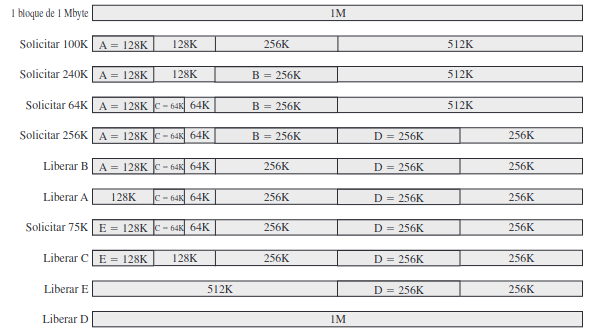
\includegraphics[width=15cm]{buddy.png}\par
    \caption{Ejemplo de sistema \textit{buddy} . }
\end{figure}

\subsection{Reubicación}
Cuando se utiliza el esquema de particionamiento fijo (Figura 3.a), se espera que un proceso siempre se asigne a la misma partición. Cuando el proceso se carga por primera vez, todas las referencias de la memoria relativas del código se reemplazan por direcciones de la memoria principal absolutas, determinadas por la dirección base del proceso cargado.\\\\ 
En el caso de particiones de igual tamaño (Figura 2) y en el caso de una única cola de procesos para particiones de distinto tamaño (Figura 3.b), un proceso puede ocupar diferentes particiones durante su ciclo de vida. Por lo tanto, las ubicaciones (de instrucciones y datos) referenciadas por un proceso no son fijas. Para resolver este problema, se realiza una distinción entre tipos de direcciones. Una \textbf{dirección lógica} es una referencia a una ubicación de memoria independiente de la asignación actual de datos a la memoria; se debe llevar a cabo una traducción a una dirección física antes de alcanzar el acceso a la memoria. Una \textbf{dirección relativa} es un ejemplo particular de dirección lógica, en la que es expresada como una ubicación relativa a algún punto conocido, normalmente un valor en un registro del procesador. Una \textbf{dirección física}, o dirección absoluta es una ubicación real de la memoria principal. \\\\ 
Los programas que emplean direcciones relativas de memoria se cargan utilizando carga dinámica en tiempo de ejecución. Normalmente, todas las referencias de memoria de los procesos cargados son relativas al origen del programa. Por tanto, se necesita un mecanismo de hardware para traducir las direcciones relativas a direcciones físicas de la memoria principal, en tiempo de ejecución de la instrucción que contiene a dicha referencia. \\\\ 
Cuando un proceso se asigna al estado ejecutando, un registro especial del procesador, llamado registro base, carga la dirección inicial del programa en la memoria principal. Existe un registro \textbf{valla} que indica el final de la ubicación del programa; estos valores se establecen cuando el programa se carga en la memoria cuando la imagen del proceso se lleva a la memoria. A lo largo de la ejecución del proceso, se encuentran direcciones relativas. Estas incluyen los contenidos del registro de las instrucciones, las direcciones de instrucciones que ocurren en los saltos e instrucciones \textit{call}, y direcciones de datos existentes en instrucciones de carga y almacenamiento. El procesador manipula cada dirección relativa, a través de dos pasos. Primero, el valor del registro base se suma a la dirección relativa para producir una dirección absoluta. Segundo, la dirección resultante se compara con el valor del registro \textbf{valla} . Si la dirección se encuentra dentro de los límites, entonces se puede llevar a cabo la ejecución de la instrucción. En otro caso, se genera una interrupción, que debe manejar el sistema operativo de algún modo. \\\\ 
El esquema de la Figura 6 permite que se traigan a memoria los programas y que se lleven a disco, a lo largo de la ejecución. También proporcionan una medida de protección: cada imagen del proceso está asilada mediante los contenidos de los registros base y valla. Además, evita accesos no autorizados por parte de otros procesos.
\begin{figure}[H]
    \centering
    \includegraphics[width=15cm]{reubicación.png}
    \caption{Soporte hardware para la reubicación.}
\end{figure}
\section{Paginación}
Supóngase que la memoria principal se divide en porciones de tamaño fijo relativamente pequeños, y que cada proceso también se divide en porciones pequeñas del mismo tamaño fijo. A dichas porciones del proceso, denominadas \textbf{páginas}, se les asigna porciones disponibles de memoria, denominadas \textbf{marcos} o marcos de páginas. Esta sección muestra que el espacio de memoria malgastado por cada proceso debido a la fragmentación interna corresponde solo a una fracción de la última página de un proceso.
\begin{tcolorbox}[colback=cyan!10, colframe=blue!70, title=Nota]
    No existe fragmentación externa.
\end{tcolorbox}
\begin{figure}[H]
    \centering
    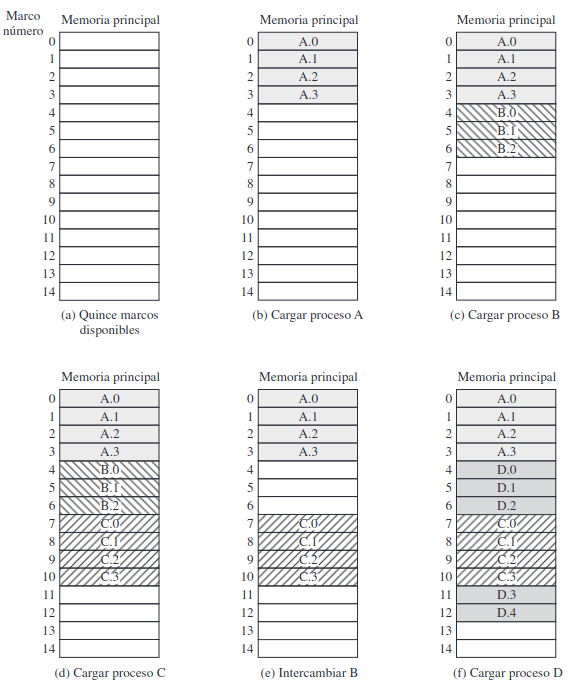
\includegraphics[width=15cm]{marco.png}
    \caption{Asignación de páginas de proceso a marcos libres}
\end{figure}
La figura 7 ilustra el uso de páginas y marcos. En un momento dado, los marcos de la memoria están en uso y algunos están libres. El sistema operativo mantiene una lista de marcos libres. El proceso A, almacenado en disco, está formado por cuatro páginas. En el momento de cargar este proceso, el sistema operativo encuentra cuatro marcos libres y carga las cuatro páginas del proceso A en dichos marcos (Figura 7.b). El proceso B, formado por tres páginas, y el proceso C, formado por cuatro páginas, se cargan a continuación. En ese momento, el proceso B se suspende y deja la memoria principal. Posteriormente, todos los procesos de la memoria principal se bloquean, y el sistema operativo necesita traer un nuevo proceso, el proceso D, que está formado por cinco páginas. \\\\ 
Suponiendo que no hubiera suficientes marcos contiguos sin utilizar para ubicar un proceso, esto no evitaría que el sistema operativo cargara el proceso D, debido a que el sistema operativo mantiene una \textbf{tabla de páginas} por cada proceso. La tabla de páginas muestra la ubicación del marco por cada página del proceso. Dentro del programa, cada dirección lógica está formada por un número de página y un desplazamiento dentro de la página.\\\\
Con esta paginación, la traducción de direcciones lógicas a físicas las realiza también el hardware del procesador. Para ello, el procesador utiliza la tabla de páginas para producir, a partir de una dirección lógica(número de página, desplazamiento), una dirección física (número de marco, desplazamiento).\\\\ 
Adicionalmente, el sistema operativo mantiene una única lista de marcos libres de todos los marcos de la memoria que se encuentran actualmente no ocupados y disponibles para las páginas.
\begin{figure}[H]
    \centering
    \includegraphics[width=15cm]{paginación2.png}
    \caption{Estructuras de datos para el ejemplo de la Figura 7 en el instante (f)}
\end{figure}

\section{Segmentación}
Un programa de usuarios puede subdividirse utilizando segmentación, en el cual el programa y sus datos asociados se dividen en un número de \textbf{segmentos}. No se requiere que todos los programas sean de la misma longitud, aunque hay una longitud máxima de segmento. Al igual que en el caso de la paginación, una dirección lógica estará compuesta por un número de segmento y un desplazamiento.\\\\ 
Debido al uso de segmentos de distinto tamaño, la segmentación es similar al particionamiento dinámico. En la ausencia de un esquema de \textit{overlays} o el uso de la memoria virtual, se necesitaría que todos los segmentos de un programa se cargaran en la memoria para su ejecución. La diferencia, comparada con el particionamiento dinámico, es que con la segmentación un programa podría ocupar más de una partición, y estas particiones no necesitan ser contiguas. La segmentación eliminar la fragmentación interna pero, al igual que el particionamiento dinámico, sufre de fragmentación externa. \\\\ 
Mientras que la paginación es invisible al programador, la segmentación es normalmente visible y se proporciona como una utilidad para organizar programas y datos. El inconveniente principal de este servicio es que el programador debe ser consciente de la limitación de tamaño de segmento máximo. \\\\ 
Otra consecuencia de utilizar segmentos de distinto tamaño es que no hay una relación simple entre direcciones lógicas y direcciones físicas. De forma análoga a la paginación, un esquema de segmentación sencillo haría uso de una tabla de segmentos por cada proceso y una lista de bloques libre de memoria principal. Cada entrada de la tabla de segmentos tendría que proporcionar la dirección inicial de la memoria principal del correspondiente segmento. La entrada también debería proporcionar la longitud del segmento, para asegurar que no se utilizan direcciones no válidas. \\\\ 
Con la segmentación simple, un proceso se divide en un conjunto de segmentos que no tienen que ser del mismo tamaño. Cuando un proceso se trae a memoria, todos sus segmentos se cargan en regiones de memoria disponibles, y se crea la tabla de segmentos.
\begin{figure}[H]
    \centering
    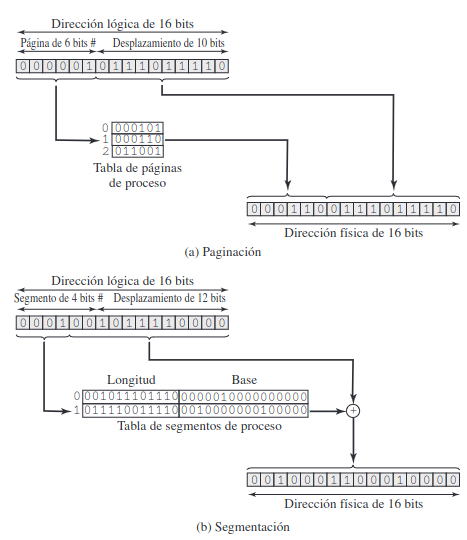
\includegraphics[width=15cm]{segmentacion.png}
    \caption{Ejemplos de traducción de direcciones lógicas a físicas.}
\end{figure}

\section{Memoria Virtual}
\subsection{Hardware y Estructuras de Control}
Las dos características de la paginación y la segmentación que son claves para este comienzo son:
\begin{enumerate}
    \item Todas las referencias a la memoria dentro de un proceso se realizan a direcciones lógicas, que se traducen dinámicamente en direcciones físicas durante la ejecución. Por lo tanto, un proceso puede ser llevado y traído a memoria de forma que ocupe diferentes regiones de la memoria principal en distintos instantes de tiempo durante la ejecución.
    \item Un proceso puede dividirse en varias porciones y estas porciones no tienen que estar localizadas en la memoria de forma contigua durante la ejecución. La combinación de la traducción en direcciones dinámicas en ejecución y el uso de una tabla de páginas o segmentos lo permite.
\end{enumerate}
\textit{Si las dos características anteriores se dan, entonces es necesario que todas las páginas todos los segmentos  de un proceso se encuentren en la memoria principal durante la ejecución.} Si la porción en la que se encuentra la siguiente instrucción a buscar está y si la porción donde se encuentra la siguiente dirección de datos que se va a acceder también está, entonces al menos la siguiente instrucción se podrá ejecutar.\\\\ 
Supóngase que se quiere traer un nuevo proceso de memoria. El sistema operativo comienza trayendo únicamente una o dos porciones, que incluye la porción inicial del programa y la porción inicial de datos sobre la cual acceden las primeras instrucciones. Esta parte del  proceso que se encuentra realmente en la memoria principal para, cualquier instante de tiempo, se denomina \textbf{conjunto residente} del proceso. Cuando el proceso está ejecutándose, las cosas ocurren de forma deseada mientras que todas las referencias a la memoria se encuentren dentro del conjunto residente. El procesador siempre es capaz de determinar si esto es cierto usando una tabla de segmentos o páginas. Si el procesador encuentra una dirección lógica que no se encuentra en la memoria principal se realiza la siguiente secuencia de acciones:
\begin{enumerate}
    \item El procesador genera una interrupción indicando un fallo de acceso a la memoria.
    \item El sistema operativo coloca al proceso interrumpido en un estado de bloqueado y toma el control.
    \item El sistema operativo realiza una petición de E/S, una lectura a disco, para traer a memoria principal la porción del proceso que contiene la dirección lógica que ha causado el fallo de acceso.
    \item Después de realizar la petición de E/S, el sistema operativo puede activar otro proceso que se ejecute mientras el disco realiza la operación de E/S.
    \item Una vez que la porción solicitada se ha traído a memoria principal, se lanza una nueva interrupción de E/S, dando control de nuevo al sistema operativo, que coloca al proceso afectado de nuevo en el estado Listo.
\end{enumerate}
Esta estrategia tiene dos grandes implicaciones o consecuencias:
\begin{enumerate}
    \item \textbf{Puede mantenerse un mayor número de procesos en memoria principal}. Debido a que solo se cargarán algunas de las porciones de los procesos a ejecutar, existe espacio para más procesos. Aumentando el nivel de multiprogramación y por consecuencia directa, un uso más eficiente del procesador.
    \item \textbf{Un proceso puede ser mayor que toda la memoria principal}. Con la memoria virtual, el trabajo de controlar cuánta memoria está disponible es delegada al sistema operativo y al hardware. En lo que concierne al programador, él está trabajando con una memoria enorme, con un tamaño asociado al almacenamiento en disco. El sistema operativo automáticamente carga porciones de un proceso en la memoria principal cuando estas se necesitan.
\end{enumerate}
Debido a que un proceso ejecuta solo en la memoria principal, esta memoria se denomina \textbf{memoria real}. Pero el programador o usuario perciben una memoria potencialmente más grande, localizada en el disco, denominada \textbf{memoria virtual}.

\begin{figure}[H]
    \centering
    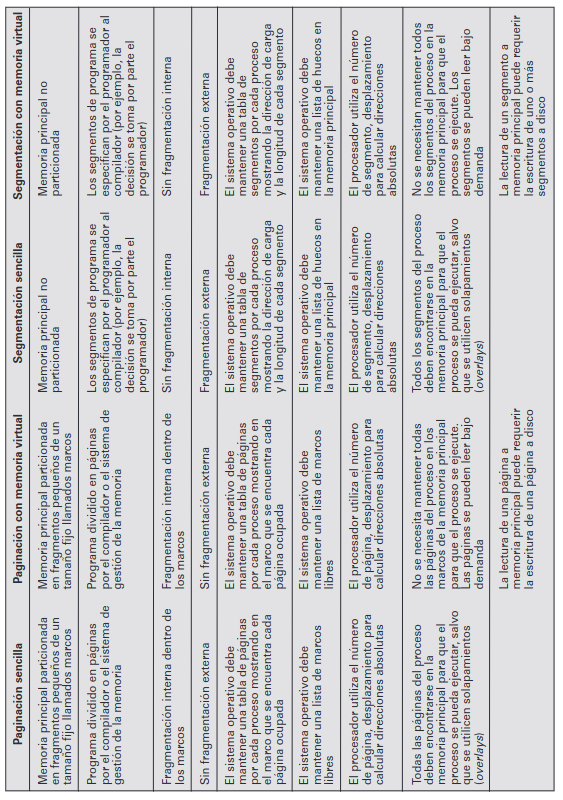
\includegraphics[width=15cm]{virtual1.png}
    \caption{Características de la paginación y segmentación.}
\end{figure}
 \subsubsection{Proximidad y Memoria Virtual}
La memoria virtual, basada en paginación o paginación más segmentación es un componente esencial de todos los sistemas operativos contemporáneos.\\\\ 
Para entender el aspecto clave, se analiza las tareas del sistema operativo relacionadas con la memoria virtual. Considerando un proceso de gran tamaño, consistente en un programa largo más un gran número de vectores de datos. A lo largo de un corto periodo de tiempo, la ejecución se puede acotar a una pequeña sección del programa y el acceso a uno o dos vectores de datos únicamente. Si es así, sería verdaderamente un desperdicio cargar docenas de porciones de dicho proceso cuando solo unas pocas se usarán antes de que el programa se suspenda o se mande a \textit{swap}. Se puede hacer un mejor uso de la memoria cargando únicamente unas pocas porciones. Entonces, si el programa salta a una destrucción o hace referencia a un dato que se encuentra en una porción de memoria que no está en la memoria principal, entonces se dispara un fallo. Este indica al sistema operativo que debe conseguir la porción deseada. \\\\ 
Así en cualquier momento, solo unas pocas porciones de cada proceso se encuentran en memoria, por lo tanto, se pueden mantener más procesos alojados en la misma. Además, se ahorra tiempo porque las porciones del proceso no usadas no se expulsarán de la memoria a \textit{swap} y de \textit{swap} a la memoria. Sin embargo, el sistema operativo debe ser inteligente a la hora de manejar este esquema. En estado estable, prácticamente toda la memoria principal se encontrará ocupada con porciones de procesos de forma que el procesador y el sistema operativo tengan acceso directo al mayor número posible de procesos. Así, cuando el sistema operativo traiga una porción a la memoria, debe expulsar otra. Si elimina una porción justo antes de que vaya a ser utilizada, deberá recuperar dicha porción de nuevo de casi forma inmediata. Un abuso de esto lleva una condición denominada \textbf{\textit{thrashing}}: el sistema consume la mayor parte del tiempo enviando y trayendo porciones de \textit{swap} en lugar de ejecutar instrucciones. Para evitar el \textit{thrashing}, el sistema operativo utiliza algoritmos complejos para tratar de adivinar, en base a la historia reciente, qué porciones son menos probables de ser utilizadas en un futuro cercano. \\\\ 
Este razonamiento se basa en la creencia del \textbf{principio de proximidad}, el cual indicia que las referencias al programa y a los datos dentro de un proceso tienden a agruparse. Por lo tanto, se resume que solo unas pocas porciones del proceso se necesitaran a lo largo de un periodo de tiempo corto.
\subsubsection{Paginación}
Para la memoria virtual basada en el esquema de paginación también se necesita una tabla de páginas. De nuevo, normalmente se asocia una única tabla de páginas a cada proceso. En este caso, sin embargo, las entradas de la tabla de páginas son más complejas. Debido a que solo algunas de las páginas de proceso se encuentran en la memoria principal, se necesita que cada entrada de la tabla de páginas indique si la correspondiente página está presente (P) en memoria principal o no. Si el bit indica que la página está en memoria, la entrada también debe indicar el número de marco de dicha página.\\\\ 
La entrada de la tabla de páginas incluye un bit de modificado (M), que indica si los contenidos de la correspondiente página han sido alterados desde que la página se cargó por última vez en la memoria principal. Si no hubo ningún cambio, no es necesario escribir la página cuando llegue el momento de reemplazarla por otra página en el marco de página que actualmente ocupa.\\\\ 
\textbf{Estructura de la tabla de páginas}. El mecanismo básico de lectura de una palabra de la memoria implica la traducción de la dirección virtual, o lógica, consistente en un número de página y un desplazamiento, a la dirección física, consistente en un número de marco y un desplazamiento, usando para ello la tabla de páginas. Debido a que la tabla de páginas es de longitud variable dependiendo del tamaño del proceso, no podemos suponer que se encuentra almacenada en los registros. En lugar de eso, debe encontrarse en la memoria principal para poder ser accedida. Cuando un proceso en particular se encuentra ejecutando, un registro contiene la dirección de comienzo de tabla de páginas para dicho proceso. El número de página de la dirección virtual se utiliza para indexar esa tabla y buscar el correspondiente marco de página. Este, combinado con la parte de desplazamiento de la dirección virtual genera la dirección real deseada. Normalmente, el campo correspondiente al número de página es mayor que el campo correspondiente al número de marco de página ($n> m$). \\\\ 
En la mayoría de sistemas, existe una única tabla de página por proceso. Pero cada proceso puede ocupar una gran cantidad de memoria virtual. Evidentemente, la cantidad de memoria demandada por las tablas de página únicamente puede ser inaceptablemente grande. Para resolver este problema, la mayoría de esquemas de memoria virtual almacena las tablas de páginas también en la memoria virtual, en lugar de en la memoria real. Esto representa que las tablas de páginas están sujetas a paginación igual que cualquier otra página. Cuando un proceso está en ejecución, al menos parte de su tabla de página debe encontrarse en memoria, incluyendo la entrada de tabla de páginas de la página actualmente en ejecución. Existes múltiples esquemas para implementar paginación en memoria virtual: \\

\textbf{Paginación de dos niveles}. Algunos procesadores utilizan un esquema de dos niveles para organizar las tablas de páginas de gran tamaño. En este esquema, existe un directorio de páginas, en el cual cada entrada apuntaba a una tabla de páginas. De esta forma, si la extensión del directorio de páginas es $X$ , y si la longitud máxima de una tabla de páginas es $Y$ , entonces un proceso consistirá en hasta $X\geq Y$ páginas. Normalmente, la longitud máxima de la tabla de páginas se restringe para que sea igual a una página. La Figura 11 muestra un ejemplo que usa 32 bits para la dirección. Asumimos un direccionamiento a nivel byte y páginas de 4 Kbytes($2^{12}$ ), por tanto, el espacio de direcciones virtuales de 4Gbytes($2^{32}$ ) se compone de $2^{20}$ . ISi cada una de estas páginas se referencia por medio de una entrada la tabla de páginas (ETP) de 4-bytes, podemos crear una tabla de página de usuario con 2^{20} la ETP que requiere 4Mbytes ($2^{22}$ bytes). Esta enorme tabla de páginas de usuario, que ocupa $2^{10}$ páginas, puede mantenerse en memoria virtual y hacerse referencia desde una tabla de páginas raíz con $2^{10}$ PTE que ocuparía 4 Kbytes($2^{12}$ ) de memoria principal. La Figura 12 muestra los pasos relacionas con la traducción de direcciones para este esquema. La página raíz siempre se mantiene en la memoria principal. Los primeros 10 bits de la dirección virtual se pueden usar para indexar en la tabla de páginas raíz para encontrar la ETP para la página en la que está la tabla de páginas de usuario. Si la página no está en la memoria principal, se produce un fallo de página. Si la página está en la memoria principal, los siguientes 10 bits de la dirección virtual se usan para indexar la tabla de páginas de usuario para encontrar la ETP de la página a la cual se hace referencia desde la dirección virtual original.\\\\ 
\begin{figure}[H]
    \centering
    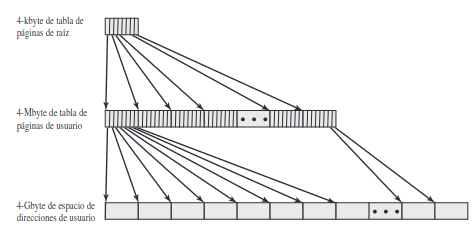
\includegraphics[width=15cm]{virtual2.png}
    \caption{Una tabla de páginas jerárquica de dos niveles}
\end{figure}
\begin{figure}[H]
    \centering
    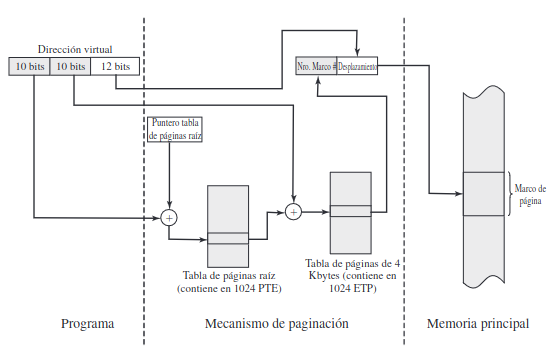
\includegraphics[width=15cm]{virtual3.png}
    \caption{Traducción de direcciones en un sistema de paginación de dos niveles.}
\end{figure}


\textbf{Tabla de páginas invertida}. Una desventaja del tipo de tablas de páginas que hemos visto es que su tamaño es proporcional al espacio de direcciones virtuales. 
\begin{figure}[H]
    \centering
    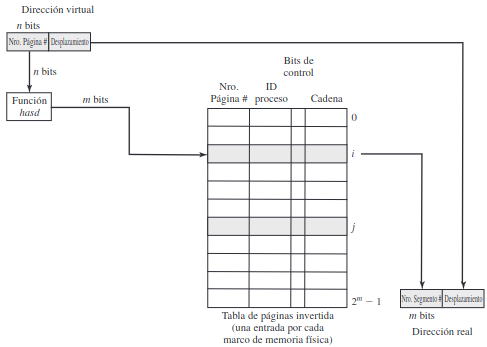
\includegraphics[width=15cm]{virtual4.png}
    \caption{Estructura de tabla de páginas invertida.}
\end{figure}
Entonces, una estrategia alternativa al uso de tablas de páginas de uno o varios niveles es el uso de la estructura de \textbf{tabla de páginas invertida}. En esta estrategia, la parte correspondiente al número de página de la dirección virtual se referencia por medio de un valor \textit{hash}, usando una función \textit{hash} sencilla. El valor \textit{hash} es un puntero para la tabla de páginas invertida, que contiene las entradas de tablas de página. Hay una entrada en la tabla de páginas invertida por cada marco de página real en lugar de uno por cada página virtual. De esta forma, lo único que se requiere para estas tablas de página siempre es una proporción fija de la memoria real, independientemente del número de procesos o de las ṕaginas virtuales soportadas. Debido a que más de una dirección virtual puede traducirse en la misma entrada de la tabla \textit{hash}, una técnica de encadenamiento se utilizan para gestionar el desbordamiento. Las técnicas de \textit{hashing}, proporcionan habitualmente cadenas que no son excesivamente largas. La estructura de la tabla de páginas se denomina invertida debido a que se indexan sus entradas de la tabla de páginas por el número de marco en lugar de por el número de página virtual. \\\\ 

La Figura 13 muestra una implementación típica de la técnica de tabla de páginas invertida. Para un tamaño de memoria física de $2^m$ marcos, la tabla de páginas invertida contiene $2^m$ entradas, de forma que la entrada en la posición \textit{i-ésima} se refiere al marco \textit{i}. La entrada en la tabla de páginas incluye la siguiente información:
\begin{itemize}
    \item \textbf{Número de página}. Esta es la parte correspondiente al número de página de la dirección virtual.
    \item \textbf{Identificador del proceso}. El proceso que es propietario de esta página. La combinación de número de página e identificador del proceso identifica a una página dentro del espacio de direcciones virtual de un proceso en particular.
    \item \textbf{Bits de control}. Este campo incluye los \textit{flags}, como por ejemplo, válido, referenciado y modificado; e información de protección y cerrojos.
\item \textbf{Puntero de la cadena}. Este campo es nulo (indicado posiblemente por un bit adicional) si no hay más entradas encadenadas en esta entrada. En otro caso este campo contiene el valor del índice (número entre $0$ y $2^{m-1}$) de la siguiente entrada de la cadena.
\end{itemize}
En este ejemplo, la dirección virtual incluye un número de página de $n$ bits, con $n > m$. La función \textit{hash} traduce el número de página \textit{n bits}, que se utiliza para indexar en la tabla de páginas invertida.


\section {Bibliografía}
\begin{itemize}
    \item Stallings, W. (2005). Sistemas operativos. Aspectos internos y principios de diseño (Quinta ed.). Pearson Education.
\end{itemize}

\end{document}
